\documentclass[aspectratio=169,12pt]{beamer}

% Theme
\usetheme{Madrid}
\usecolortheme{whale}
\setbeamertemplate{navigation symbols}{}
\setbeamertemplate{footline}[frame number]
\setbeamercolor{frametitle}{bg=structure.fg!15!bg}

% Packages
\usepackage{graphicx}
\usepackage{booktabs}
\usepackage{tikz}
\usepackage{fontspec}
\usepackage{listings}
\usepackage{xcolor}
\usepackage{hyperref}

% Code style
\lstset{
  basicstyle=\ttfamily\small,
  keywordstyle=\color{blue}\bfseries,
  stringstyle=\color{red!70!black},
  commentstyle=\color{green!50!black}\itshape,
  breaklines=true,
  frame=single,
  backgroundcolor=\color{gray!10},
  language=Python,
  showstringspaces=false,
}

% Colors
\definecolor{ubuntupurple}{RGB}{119,41,83}
\definecolor{ubuntuorange}{RGB}{233,84,32}
\definecolor{predictblue}{RGB}{41,98,255}
\definecolor{gengreen}{RGB}{0,150,80}

% Title info
\title[Predictive to Generative AI]{From Predictive to Generative AI}
\subtitle{A Hands-On Journey Through the AI Revolution}
\author{UbuCon 2026 Workshop}
\date{}
\institute{}

\begin{document}

% ============================================================
% TITLE SLIDE
% ============================================================
\begin{frame}
\titlepage
\end{frame}

% ============================================================
% OPENING (5 min)
% ============================================================
\begin{frame}{What We'll Build Today}
\begin{columns}
\begin{column}{0.5\textwidth}
\textbf{Three Notebooks, One Story:}
\begin{enumerate}
\item \textcolor{predictblue}{\textbf{Predictive AI}} --- Traditional ML
\item \textcolor{gengreen}{\textbf{Generative AI}} --- LLMs \& Chat
\item \textcolor{ubuntupurple}{\textbf{AI kwa Kiswahili}} --- Your Language
\end{enumerate}
\vspace{0.5cm}
\textbf{You'll leave with:}
\begin{itemize}
\item Working code you can reuse
\item Skills to choose the right AI approach
\item AI running locally on Ubuntu
\end{itemize}
\end{column}
\begin{column}{0.5\textwidth}
\begin{center}
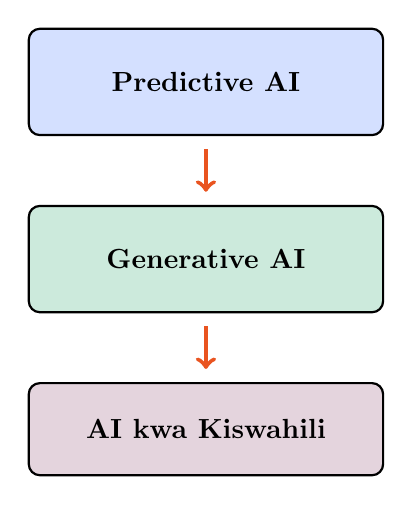
\begin{tikzpicture}[scale=0.9]
\draw[fill=predictblue!20, rounded corners, thick] (0,4) rectangle (5,5.5);
\node[font=\bfseries] at (2.5,4.75) {Predictive AI};
\draw[->, ultra thick, ubuntuorange] (2.5,3.8) -- (2.5,3.2);
\draw[fill=gengreen!20, rounded corners, thick] (0,1.5) rectangle (5,3);
\node[font=\bfseries] at (2.5,2.25) {Generative AI};
\draw[->, ultra thick, ubuntuorange] (2.5,1.3) -- (2.5,0.7);
\draw[fill=ubuntupurple!20, rounded corners, thick] (0,-.8) rectangle (5,0.5);
\node[font=\bfseries] at (2.5,-0.15) {AI kwa Kiswahili};
\end{tikzpicture}
\end{center}
\end{column}
\end{columns}
\end{frame}

\begin{frame}{Workshop Flow}
\begin{center}
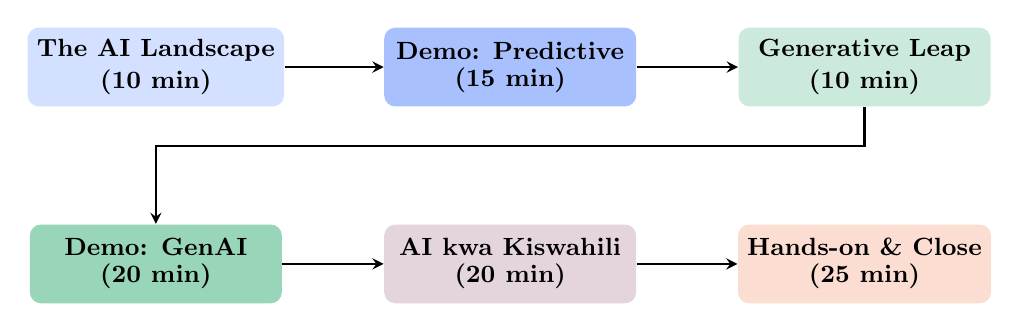
\begin{tikzpicture}[
  block/.style={rectangle, rounded corners, minimum width=3.2cm, minimum height=1cm, text centered, font=\small\bfseries},
  arrow/.style={->, thick, >=stealth}
]
\node[block, fill=predictblue!20] (a) at (0,0) {\shortstack{The AI Landscape\\(10 min)}};
\node[block, fill=predictblue!40] (b) at (4.5,0) {\shortstack{Demo: Predictive\\(15 min)}};
\node[block, fill=gengreen!20] (c) at (9,0) {\shortstack{Generative Leap\\(10 min)}};
\node[block, fill=gengreen!40] (d) at (0,-2.5) {\shortstack{Demo: GenAI\\(20 min)}};
\node[block, fill=ubuntupurple!20] (e) at (4.5,-2.5) {\shortstack{AI kwa Kiswahili\\(20 min)}};
\node[block, fill=ubuntuorange!20] (f) at (9,-2.5) {\shortstack{Hands-on \& Close\\(25 min)}};

\draw[arrow] (a) -- (b);
\draw[arrow] (b) -- (c);
\draw[arrow] (c) -- ++(0,-1) -| (d);
\draw[arrow] (d) -- (e);
\draw[arrow] (e) -- (f);
\end{tikzpicture}
\end{center}
\vspace{0.3cm}
\begin{center}
\textit{Total: 1 hour 45 minutes --- slides + live coding + hands-on}
\end{center}
\end{frame}

% ============================================================
% THE AI LANDSCAPE (10 min)
% ============================================================
\begin{frame}{Two Worlds of AI}
\begin{columns}
\begin{column}{0.45\textwidth}
\begin{center}
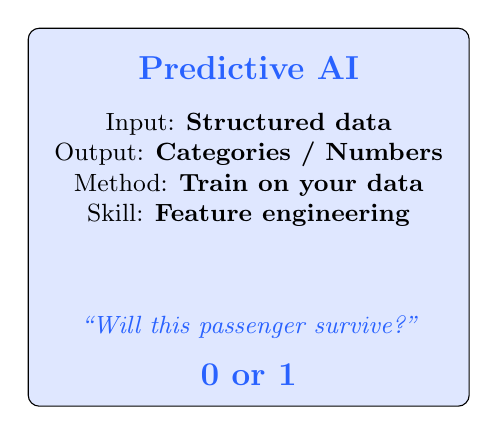
\begin{tikzpicture}
\draw[fill=predictblue!15, rounded corners] (-2.8,-2) rectangle (2.8,2.8);
\node[font=\large\bfseries, predictblue] at (0,2.3) {Predictive AI};
\node[align=center, font=\small] at (0,1) {
  Input: \textbf{Structured data}\\
  Output: \textbf{Categories / Numbers}\\
  Method: \textbf{Train on your data}\\
  Skill: \textbf{Feature engineering}
};
\node[font=\small\itshape, predictblue] at (0,-1) {``Will this passenger survive?''};
\node[font=\large\bfseries, predictblue] at (0,-1.6) {0 or 1};
\end{tikzpicture}
\end{center}
\end{column}
\begin{column}{0.08\textwidth}
\begin{center}
{\Huge\textcolor{ubuntuorange}{$\rightarrow$}}
\end{center}
\end{column}
\begin{column}{0.45\textwidth}
\begin{center}
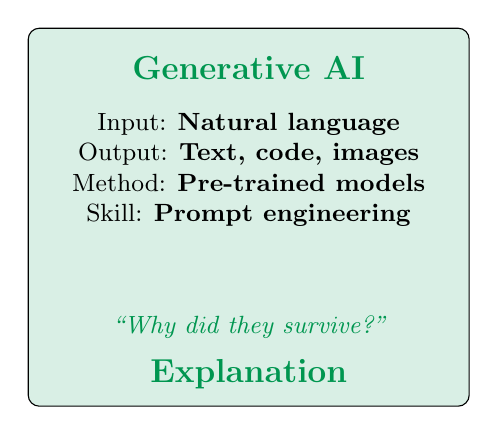
\begin{tikzpicture}
\draw[fill=gengreen!15, rounded corners] (-2.8,-2) rectangle (2.8,2.8);
\node[font=\large\bfseries, gengreen] at (0,2.3) {Generative AI};
\node[align=center, font=\small] at (0,1) {
  Input: \textbf{Natural language}\\
  Output: \textbf{Text, code, images}\\
  Method: \textbf{Pre-trained models}\\
  Skill: \textbf{Prompt engineering}
};
\node[font=\small\itshape, gengreen] at (0,-1) {``Why did they survive?''};
\node[font=\large\bfseries, gengreen] at (0,-1.6) {Explanation};
\end{tikzpicture}
\end{center}
\end{column}
\end{columns}
\end{frame}

\begin{frame}{The Paradigm Shift}
\begin{center}
\renewcommand{\arraystretch}{1.4}
\begin{tabular}{l c c}
\toprule
& \textcolor{predictblue}{\textbf{Predictive AI}} & \textcolor{gengreen}{\textbf{Generative AI}} \\
\midrule
\textbf{You write} & Code \& features & Prompts \\
\textbf{Model learns from} & Your labeled data & Internet-scale data \\
\textbf{Output} & Numbers & Language \\
\textbf{Strength} & Precise, measurable & Flexible, creative \\
\textbf{Weakness} & Only predicts known categories & Can hallucinate \\
\textbf{Example} & ``Survived'' / ``Died'' & ``She survived because\ldots'' \\
\bottomrule
\end{tabular}
\end{center}
\vspace{0.5cm}
\begin{center}
\Large\textbf{Neither is better --- they solve different problems.}
\end{center}
\end{frame}

\begin{frame}{The Traditional ML Pipeline}
\begin{center}
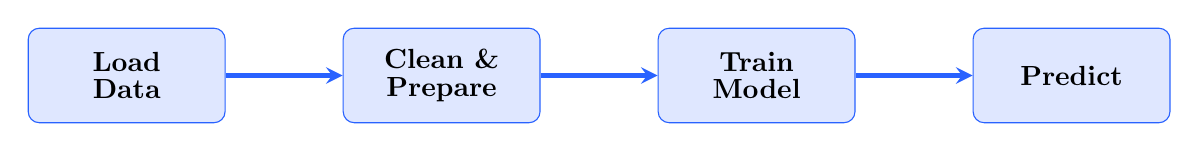
\begin{tikzpicture}[
  box/.style={rectangle, rounded corners, draw=predictblue, fill=predictblue!15, minimum width=2.5cm, minimum height=1.2cm, text centered, font=\bfseries},
  arrow/.style={->, ultra thick, predictblue, >=stealth}
]
\node[box] (load) at (0,0) {\shortstack{Load\\Data}};
\node[box] (clean) at (4,0) {\shortstack{Clean \&\\Prepare}};
\node[box] (train) at (8,0) {\shortstack{Train\\Model}};
\node[box] (predict) at (12,0) {Predict};

\draw[arrow] (load) -- (clean);
\draw[arrow] (clean) -- (train);
\draw[arrow] (train) -- (predict);
\end{tikzpicture}
\end{center}
\vspace{0.8cm}
\begin{itemize}
\item \textbf{Dataset}: Titanic --- 891 passengers, 7 features
\item \textbf{Algorithm}: Logistic Regression
\item \textbf{Goal}: Predict survived (1) or died (0)
\item \textbf{Limitation}: Can \textit{only} output 0 or 1 --- no explanations
\end{itemize}
\end{frame}

% ============================================================
% LIVE DEMO 1 TRANSITION
% ============================================================
\begin{frame}[plain]
\begin{center}
\vspace{2cm}
{\Huge\textcolor{predictblue}{\textbf{Live Demo}}}\\[0.5cm]
{\LARGE Notebook 1: Predictive AI}\\[0.3cm]
{\large Titanic Classification with Logistic Regression}\\[1cm]
{\normalsize Load $\rightarrow$ Clean $\rightarrow$ Train $\rightarrow$ Predict}\\[1.5cm]
\textit{\small Switch to: \texttt{01\_Predictive\_AI\_Titanic.ipynb}}
\end{center}
\end{frame}

% ============================================================
% THE GENERATIVE LEAP (10 min)
% ============================================================
\begin{frame}{The Limitation We Just Hit}
\begin{center}
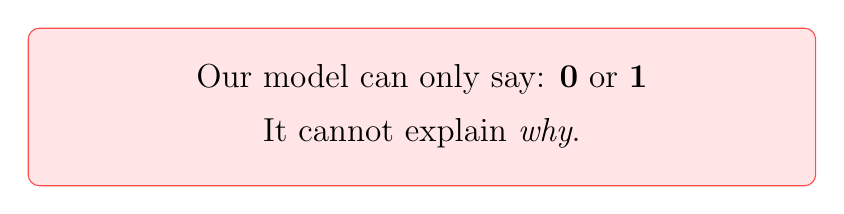
\begin{tikzpicture}
\node[rectangle, rounded corners, draw=red!70, fill=red!10, minimum width=10cm, minimum height=2cm, font=\large] at (0,0) {
  \begin{tabular}{c}
  Our model can only say: \textbf{0} or \textbf{1}\\[0.2cm]
  It cannot explain \textit{why}.
  \end{tabular}
};
\end{tikzpicture}
\end{center}
\vspace{0.5cm}
\textbf{What if we could ask:}
\begin{itemize}
\item ``\textit{Why} did this passenger survive?''
\item ``What \textit{patterns} do you see in the data?''
\item ``Write a \textit{survival guide} for 1912 passengers''
\item ``Explain this in \textit{Kiswahili}''
\end{itemize}
\vspace{0.3cm}
\begin{center}
\Large This is what \textcolor{gengreen}{\textbf{Generative AI}} unlocks.
\end{center}
\end{frame}

\begin{frame}{Prompt Engineering --- The New Programming}
\begin{center}
\renewcommand{\arraystretch}{1.5}
\begin{tabular}{l l l}
\toprule
\textbf{Component} & \textbf{Purpose} & \textbf{Example} \\
\midrule
\textbf{Role} & Who the AI is & ``You are a Titanic historian'' \\
\textbf{Context} & Background info & ``891 passengers, 38\% survived'' \\
\textbf{Task} & What to do & ``Predict survival'' \\
\textbf{Format} & How to answer & ``Reply: SURVIVED or DIED'' \\
\bottomrule
\end{tabular}
\end{center}
\vspace{0.5cm}
\begin{center}

\begin{tikzpicture}
\node[rectangle, rounded corners, draw=gengreen, fill=gengreen!10, minimum width=9cm, minimum height=1.2cm, font=\large] at (0,0) {
  Better prompt = Better result
};
\end{tikzpicture}
\end{center}
\end{frame}

\begin{frame}{Local AI vs Cloud AI}
\begin{columns}
\begin{column}{0.48\textwidth}
\begin{center}
\textcolor{ubuntupurple}{\large\textbf{Ollama (Local)}}
\end{center}
\begin{itemize}
\item \textbf{Privacy}: Data stays on your machine
\item \textbf{Cost}: Free forever
\item \textbf{Offline}: No internet needed
\item \textbf{Ubuntu-native}: Runs best on Linux
\end{itemize}
\vspace{0.2cm}
{\small\texttt{curl -fsSL https://ollama.ai/install.sh | sh}}
\end{column}
\begin{column}{0.04\textwidth}
\rule{0.5pt}{4cm}
\end{column}
\begin{column}{0.48\textwidth}
\begin{center}
\textcolor{ubuntuorange}{\large\textbf{Gemini (Cloud)}}
\end{center}
\begin{itemize}
\item \textbf{Power}: State-of-the-art models
\item \textbf{Speed}: Google's infrastructure
\item \textbf{Free tier}: Generous limits
\item \textbf{Multimodal}: Text, images, code
\end{itemize}
\vspace{0.2cm}
{\small\texttt{pip install google-generativeai}}
\end{column}
\end{columns}
\end{frame}

\begin{frame}{The Reliability Pattern}
\begin{columns}
\begin{column}{0.45\textwidth}
\begin{center}
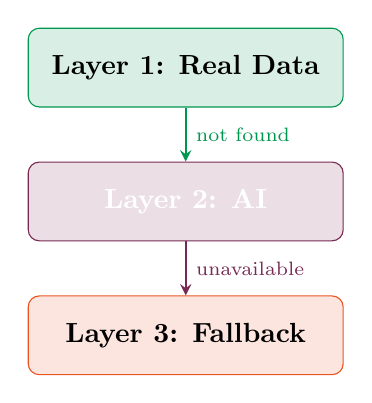
\begin{tikzpicture}[
  box/.style={rectangle, rounded corners, minimum width=4cm, minimum height=1cm, text centered, font=\bfseries},
  arrow/.style={->, thick, >=stealth}
]
\node[box, draw=gengreen, fill=gengreen!15] (data) at (0,2.5) {Layer 1: Real Data};
\node[box, draw=ubuntupurple, fill=ubuntupurple!15, text=white] (ai) at (0,0.8) {Layer 2: AI};
\node[box, draw=ubuntuorange, fill=ubuntuorange!15] (rules) at (0,-0.9) {Layer 3: Fallback};

\draw[arrow, gengreen] (data) -- node[right, font=\scriptsize] {not found} (ai);
\draw[arrow, ubuntupurple] (ai) -- node[right, font=\scriptsize] {unavailable} (rules);
\end{tikzpicture}
\end{center}
\end{column}
\begin{column}{0.52\textwidth}
\textbf{Layer 1: Real Data}\\
{\small Answer from actual statistics}\\[0.3cm]
\textbf{Layer 2: AI (Ollama $\rightarrow$ Gemini)}\\
{\small Local first, cloud as backup}\\[0.3cm]
\textbf{Layer 3: Rule-based Fallback}\\
{\small Always works, no dependencies}
\end{column}
\end{columns}
\vspace{0.4cm}
\begin{center}
\textit{The best AI systems always have a fallback.}
\end{center}
\end{frame}

% ============================================================
% LIVE DEMO 2 TRANSITION
% ============================================================
\begin{frame}[plain]
\begin{center}
\vspace{2cm}
{\Huge\textcolor{gengreen}{\textbf{Live Demo}}}\\[0.5cm]
{\LARGE Notebook 2: Generative AI}\\[0.3cm]
{\large Ollama + Gemini + Interactive Chat}\\[1cm]
{\normalsize Prompt $\rightarrow$ Generate $\rightarrow$ Evaluate $\rightarrow$ Refine}\\[1.5cm]
\textit{\small Switch to: \texttt{02\_Generative\_AI\_Demo.ipynb}}
\end{center}
\end{frame}

% ============================================================
% AI KWA KISWAHILI (5 min slides)
% ============================================================
\begin{frame}{AI kwa Kiswahili}
\begin{center}
{\Large\textcolor{ubuntupurple}{\textbf{Lugha yetu ina nafasi katika ulimwengu wa AI}}}
\end{center}
\vspace{0.5cm}
\begin{columns}
\begin{column}{0.5\textwidth}
\textbf{The Problem:}
\begin{itemize}
\item Most AI is built for English
\item 200M+ Kiswahili speakers
\item African languages underrepresented
\item Local context matters
\end{itemize}
\end{column}
\begin{column}{0.5\textwidth}
\textbf{The Solution:}
\begin{itemize}
\item Modern LLMs understand Kiswahili
\item One instruction changes everything:
\end{itemize}
\vspace{0.3cm}
\begin{center}
\fbox{\parbox{5cm}{\centering\textit{``LAZIMA ujibu kwa\\Kiswahili sanifu''}}}
\end{center}
\end{column}
\end{columns}
\vspace{0.5cm}
\begin{center}
\textbf{Same AI, same data, your language.}
\end{center}
\end{frame}

\begin{frame}{Kiswahili Prompt Engineering}
\begin{center}
{\small
\renewcommand{\arraystretch}{1.4}
\begin{tabular}{l l}
\toprule
\textbf{Kipengele} & \textbf{Mfano} \\
\midrule
\textbf{Jukumu} (Role) & ``Wewe ni mtaalamu wa historia'' \\
\textbf{Muktadha} (Context) & ``Abiria 891, 38\% walinusurika'' \\
\textbf{Kazi} (Task) & ``Eleza sababu za kunusurika'' \\
\textbf{Muundo} (Format) & ``Jibu kwa vidokezo vitatu'' \\
\textbf{Lugha} (Language) & ``Jibu kwa Kiswahili sanifu'' \\
\bottomrule
\end{tabular}
}
\end{center}
\vspace{0.3cm}
\begin{center}
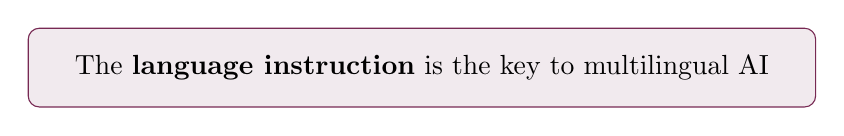
\begin{tikzpicture}
\node[rectangle, rounded corners, draw=ubuntupurple, fill=ubuntupurple!10, minimum width=10cm, minimum height=1cm, font=\normalsize] at (0,0) {
  The \textbf{language instruction} is the key to multilingual AI
};
\end{tikzpicture}
\end{center}
\end{frame}

% ============================================================
% LIVE DEMO 3 TRANSITION
% ============================================================
\begin{frame}[plain]
\begin{center}
\vspace{2cm}
{\Huge\textcolor{ubuntupurple}{\textbf{Live Demo}}}\\[0.5cm]
{\LARGE Notebook 3: AI kwa Kiswahili}\\[0.3cm]
{\large Uliza Data kwa Lugha Yako}\\[1cm]
{\normalsize zungumza(``Kwa nini wanawake walinusurika zaidi?'')}\\[1.5cm]
\textit{\small Switch to: \texttt{03\_Generative\_AI\_Kiswahili.ipynb}}
\end{center}
\end{frame}

% ============================================================
% CHOOSING THE RIGHT AI (10 min)
% ============================================================
\begin{frame}{When to Use What}
\begin{center}
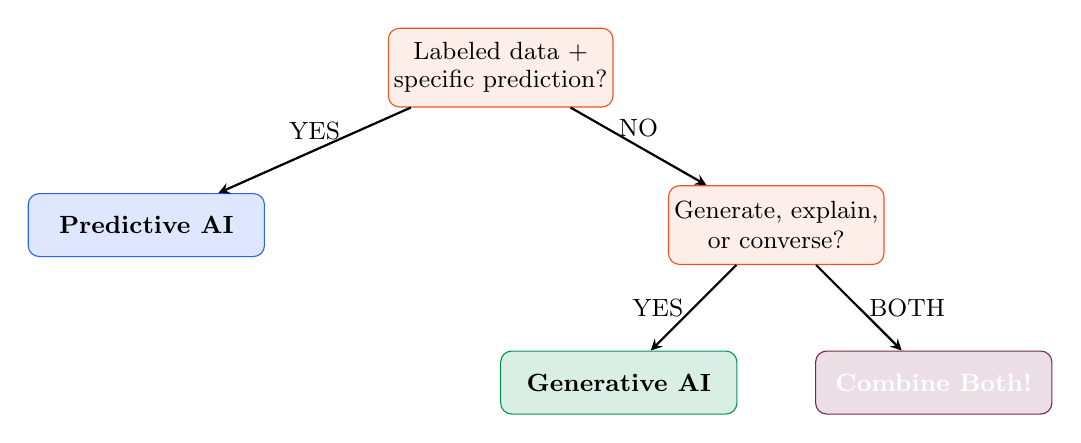
\begin{tikzpicture}[
  decision/.style={rectangle, rounded corners, draw=ubuntuorange, fill=ubuntuorange!10, minimum width=2.5cm, minimum height=1cm, text centered, font=\small, inner sep=2pt},
  result/.style={rectangle, rounded corners, minimum width=3cm, minimum height=0.8cm, text centered, font=\small\bfseries},
  arrow/.style={->, thick, >=stealth}
]
\node[decision] (q1) at (0,2) {\shortstack{Labeled data +\\specific prediction?}};
\node[result, draw=predictblue, fill=predictblue!15] (pred) at (-4.5,0) {Predictive AI};
\node[decision] (q2) at (3.5,0) {\shortstack{Generate, explain,\\or converse?}};
\node[result, draw=gengreen, fill=gengreen!15] (gen) at (1.5,-2) {Generative AI};
\node[result, draw=ubuntupurple, fill=ubuntupurple!15, text=white] (both) at (5.5,-2) {Combine Both!};

\draw[arrow] (q1) -- node[above, font=\small] {YES} (pred);
\draw[arrow] (q1) -- node[above, font=\small] {NO} (q2);
\draw[arrow] (q2) -- node[left, font=\small] {YES} (gen);
\draw[arrow] (q2) -- node[right, font=\small] {BOTH} (both);
\end{tikzpicture}
\end{center}
\vspace{0.5cm}
\begin{center}
\large\textbf{The winning pattern:}\\
Predictive AI for the numbers. Generative AI for the narrative.
\end{center}
\end{frame}

\begin{frame}{The Ubuntu Advantage}
\begin{center}
{\Large Why Ubuntu is the best platform for AI}
\end{center}
\vspace{0.5cm}
\begin{columns}
\begin{column}{0.5\textwidth}
\textbf{For Local AI:}
\begin{itemize}
\item Ollama runs natively on Linux
\item Full GPU support out of the box
\item No licensing costs
\item Docker \& containers ready
\item Privacy by default
\end{itemize}
\end{column}
\begin{column}{0.5\textwidth}
\textbf{For Development:}
\begin{itemize}
\item Python ecosystem is native
\item Package management with pip/conda
\item Jupyter runs seamlessly
\item Cloud deployment (most servers run Linux)
\item Community \& documentation
\end{itemize}
\end{column}
\end{columns}
\vspace{0.5cm}
\begin{center}
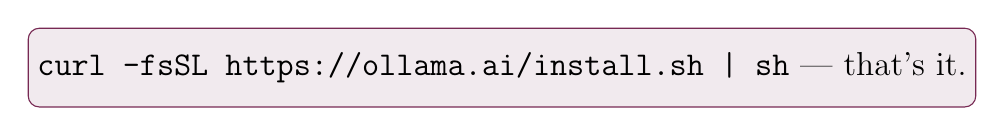
\begin{tikzpicture}
\node[rectangle, rounded corners, draw=ubuntupurple, fill=ubuntupurple!10, minimum width=10cm, minimum height=1cm, font=\large] at (0,0) {
  \texttt{curl -fsSL https://ollama.ai/install.sh | sh} --- that's it.
};
\end{tikzpicture}
\end{center}
\end{frame}

\begin{frame}{Responsible AI}
\begin{columns}
\begin{column}{0.5\textwidth}
\textbf{Always Consider:}
\begin{itemize}
\item \textbf{Hallucinations}: Convincing but wrong
\item \textbf{Bias}: Reflects training data
\item \textbf{Privacy}: Cloud sends data externally
\item \textbf{Verification}: Always validate outputs
\end{itemize}
\end{column}
\begin{column}{0.5\textwidth}
\textbf{Best Practices:}
\begin{itemize}
\item Use Ollama for sensitive data
\item Never trust AI output blindly
\item Build fallback systems
\item Test with diverse inputs
\item Be transparent about AI use
\end{itemize}
\end{column}
\end{columns}
\vspace{0.3cm}
\begin{center}
\textit{AI is a powerful tool --- use it responsibly.}
\end{center}
\end{frame}

% ============================================================
% HANDS-ON TRANSITION
% ============================================================
\begin{frame}[plain]
\begin{center}
\vspace{1.5cm}
{\Huge\textcolor{ubuntuorange}{\textbf{Your Turn!}}}\\[0.4cm]
{\LARGE Hands-On Experimentation}\\[0.5cm]
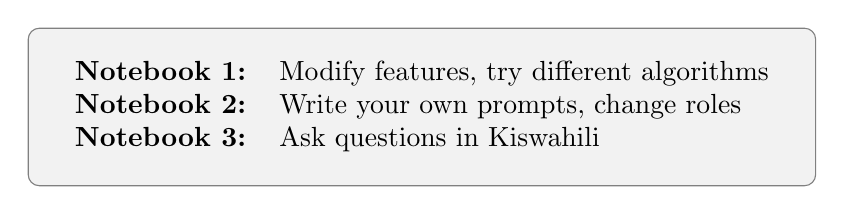
\begin{tikzpicture}
\node[rectangle, rounded corners, draw=gray, fill=gray!10, minimum width=10cm, minimum height=2cm] at (0,0) {
  \begin{tabular}{l l}
  \textbf{Notebook 1:} & Modify features, try different algorithms \\
  \textbf{Notebook 2:} & Write your own prompts, change roles \\
  \textbf{Notebook 3:} & Ask questions in Kiswahili \\
  \end{tabular}
};
\end{tikzpicture}
\\[0.4cm]
\textit{Ask questions! Experiment! Break things!}
\end{center}
\end{frame}

% ============================================================
% CLOSING (5 min)
% ============================================================
\begin{frame}{What You Learned Today}
\begin{enumerate}
\item \textcolor{predictblue}{\textbf{Predictive AI}} follows: Load $\rightarrow$ Clean $\rightarrow$ Train $\rightarrow$ Predict
\item \textcolor{gengreen}{\textbf{Generative AI}} follows: Prompt $\rightarrow$ Generate $\rightarrow$ Evaluate $\rightarrow$ Refine
\item \textbf{Prompt engineering} is the new programming
\item \textbf{Local AI} on Ubuntu gives you privacy and control
\item \textbf{Cloud AI} gives you power and convenience
\item \textbf{AI works in Kiswahili} --- your language has a place in AI
\item The \textbf{fallback pattern} makes your apps reliable
\item \textbf{Neither approach is better} --- combine them
\end{enumerate}
\end{frame}

\begin{frame}{Your AI Toolkit}
\begin{center}
{\small
\renewcommand{\arraystretch}{1.3}
\begin{tabular}{l l l}
\toprule
\textbf{Tool} & \textbf{Type} & \textbf{Link} \\
\midrule
Ollama & Local LLM & ollama.ai \\
LM Studio & Local GUI & lmstudio.ai \\
Hugging Face & Open models & huggingface.co \\
Google AI Studio & Gemini API & makersuite.google.com \\
scikit-learn & Traditional ML & scikit-learn.org \\
\bottomrule
\end{tabular}
}
\end{center}
\vspace{0.4cm}
\begin{center}
\textbf{Learning Resources:}\\
{\small Prompt Engineering Guide $\cdot$ Fast.ai $\cdot$ AI for Everyone}
\end{center}
\end{frame}

\begin{frame}[plain]
\begin{center}
\vspace{2cm}
{\Huge\textbf{Asante Sana!}}\\[0.5cm]
{\LARGE Thank You!}\\[1cm]
{\large From Predictive to Generative AI}\\[0.3cm]
{\large UbuCon 2026}\\[1.5cm]
{\normalsize\textit{Now go build something amazing.}}
\end{center}
\end{frame}

\end{document}
